\documentclass[letterpaper, 12pt]{article}

\usepackage{graphicx}
\usepackage{longtable}
\usepackage{rotating}
\usepackage{dcolumn}
\usepackage{listings}
\usepackage{subfiles}
\usepackage{amsmath}
\usepackage{subcaption}

% Code listing commands
\lstset{language=R,
basicstyle=\scriptsize\ttfamily,
commentstyle=\ttfamily,
numbers=left,
numberstyle=\footnotesize,
stepnumber=1,
numbersep=5pt,
showspaces=false,
showstringspaces=false,
showtabs=false,
frame=single,
tabsize=2,
captionpos=b,
breaklines=true,
breakatwhitespace=false,
title=\lstname,
escapeinside={},
keywordstyle={},
morekeywords={}
}

\renewcommand\thesection{Part \Alph{section}:}
\renewcommand\thesubsection{(\roman{subsection})}

\begin{document}
\title{ARE213 Problem Set \#2B}
\author{Peter Alstone \& Frank Proulx}
\maketitle

\section{Preliminaries}

\subsection{Comparison between TU and control States}

\paragraph{Starting with simple comparisons}
We begin with simple comparisons between the dependent outcome of interest, the natural logarithm of traffic fatalities per capita (log(fatalities per capita)), between a predefined composite treatment state ``TU" (or, state \#99), and all of the potential control states.  The mean over the period before primary seatbelt laws were adopted in the treatment state is -1.4 and the mean for the control states is -1.7, indicating approximately a 30\% lower typical fatalities rate in the treatment state than the average control state (even before the primary seatbelt law ``treatment").  The trends for both shown in Figure \ref{fig:a11} show that overall the fatalities were on the decline in both places before the treatment period.  

\paragraph{Roadmap}
Extracting meaningful conclusions from these data is the goal of our analysis, which will require identifying the variation in traffic fatalities that can be attributed to seat belt laws.  Confounding our analysis is the fact that these data are not in the context of an RCT but are from the ``real world" with messy trends and linked systems that determine outcomes.  We will be applying the synthetic controls method to identify a fleet of control states as a meaningful counterfactual to measure against for our composite treatment state.  

\begin{figure}[htbp]
\begin{center}
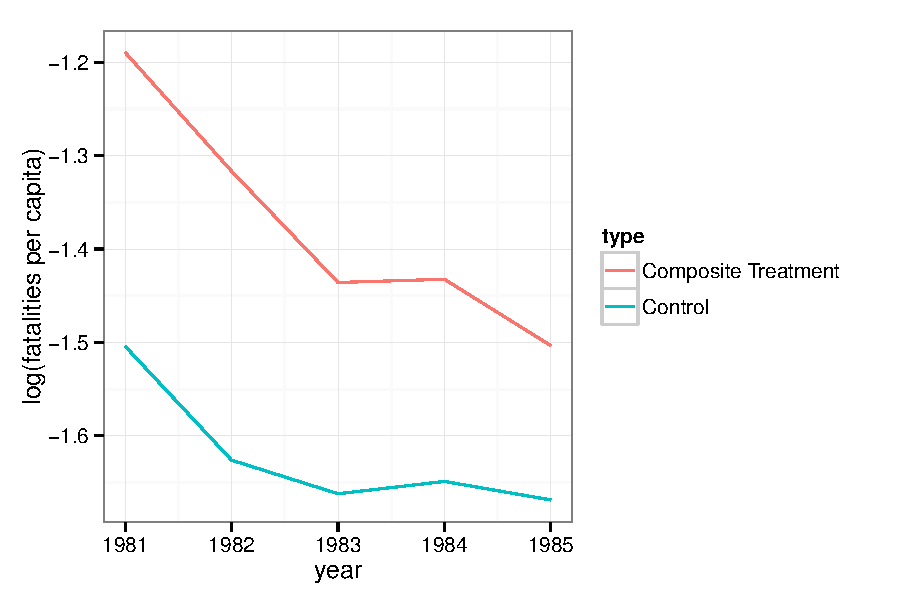
\includegraphics{img-p2b-logfatTrend.pdf}
\caption{Trend in the dependent variable (log(fatalities per capita)) for the composite treatment state and the average of the control states.}
\label{fig:a11}
\end{center}
\end{figure}


\subsection{``Best'' control state comparison}

\paragraph{Sweet Home Alabama} 
We observe that Alabama is the best match for the composite treatment state based on a simple comparison of log(fatalities per capita) in the year before treatment in the composite state (1985).  Figure \ref{fig:a21} below shows the distribution in the dependent variable 

\paragraph{Fried green covariates and other stereotypes confirmed}
Tables \ref{tab:a21} and \ref{tab:a22} compare the covariates for the composite treatment state and Alabama.  There are broad differences between the states.  Alabama has higher precipitation, lower college achievement, lower alcohol consumption, higher unemployment, etc.  Additionally, the mean value for the depdentent variable of interest, log(fatalities per capita), is quite different for the two states.  Examining the trends in the covariates (and dependent variable) for the two states (see Figure \ref{fig:a22}) shows that it could be construed as a coincidence that Alabama is the best match for the value of the dependent variable, since the trajectory in fatalities for both states are following opposite trends in that time and 1985 happens to be the time when they intersect.  There are also important and long-term differences in precipitation and alcohol consumption.  

Overall Alabama does not appear to be a particularly good match for the composite treatment state, motivating an application of synthetic controls methods to produce a better match.  

\begin{figure}[htbp]
\begin{center}
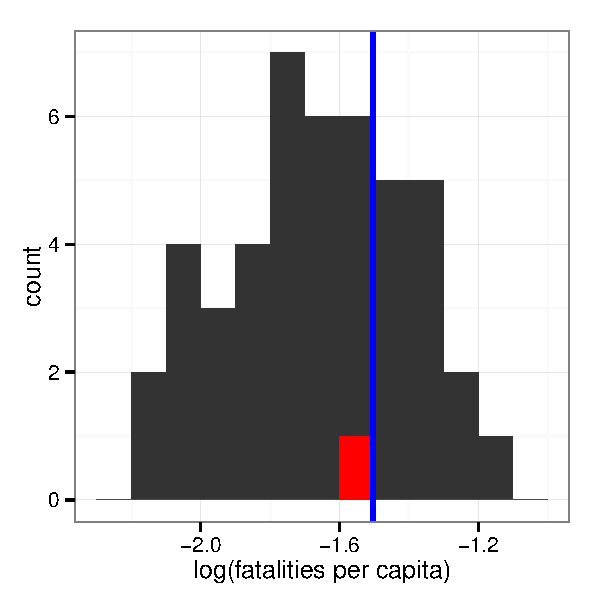
\includegraphics{img-p2b-compareStates.pdf}
\caption{Distribution in traffic fatalities metric from 1985 for all control states with a vertical blue line indicating the value of the metric for the composite treatment state.  The red block highlights the position of Alabama in the distribution.  Alabama is the closest match to the composite treatment state for 1985, but as is shown here is one of about 11 states that is within ~10\% of the target value.}
\label{fig:a21}
\end{center}
\end{figure}

\subfile{tab-ps2b-1a.tex}
\subfile{tab-ps2b-1b.tex}

\begin{figure}[htbp]
\begin{center}
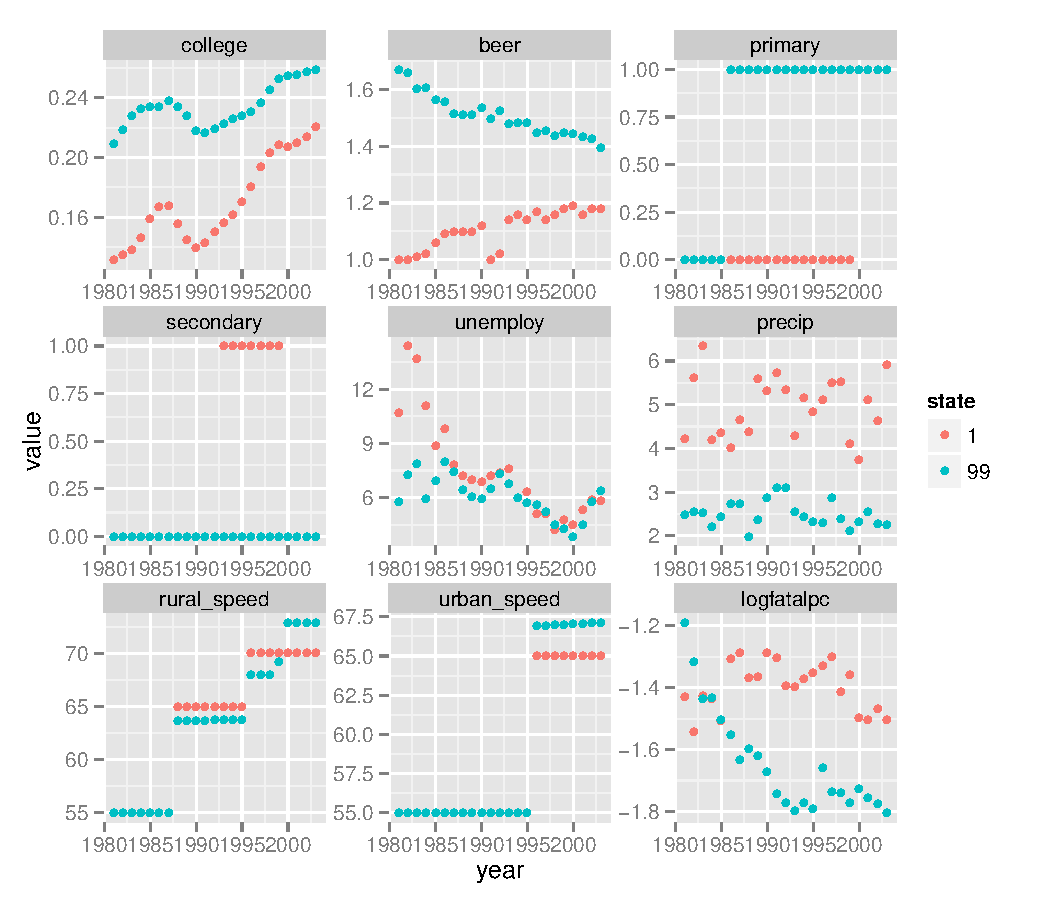
\includegraphics{img-ps2b-compareStatesFacets.pdf}
\caption{Trends in the covariate (and dependent) variables for the composite treatment state (99) and Alabama (1)}
\label{fig:a22}
\end{center}
\end{figure}


\section{Synthetic Controls}

\subsection{Why synthetic controls?}

\paragraph{Unsweet Home Alabama:}
We saw earlier the difficulties in selecting an exact counterfactual match for implementing differences in differences type selection on unobservables techniques.  While Alabama would appear on face value to be a good match (based on having similar outcomes in the year prior to treatment) we saw that this was coincidental and that the covariates are not a good match to the composite treatment state.  Synthetic control methods are motivated by producing a ``better" match by combining (synthesizing) multiple control states in a weighting scheme to create a composite control state with better match of the important covariates and dependent variable than any particular control state.  

\paragraph{Dr. Synth-love, or how I learned to stop worrying and love econometrics:}
Synthetic controls have a multi-step, iterative process for developing weighting factors to apply to control states for construction of a composite control state.  The goal is to identify a weighting matrix $W$ that minimizes the distance between the treatment covariates (e.g. alcohol consumption, total VMT) and pre-intervention outcomes (log fatalities per capita) for the weighted control unit and the treatment unit. In particular, the following more formally defined criteria are sought (from Synth R package documentation):
\begin{itemize}
\item $\sum_{j=2}^{J+1} w_j^* \bar{Y}_j^{K_1} = \bar{Y}_1^{K_M}$ , where $j$ refers to the state, $w_j$ is state $j$'s weight, and $\bar{Y}_j^{K_m}$ denotes the pre-treatment outcome in state $j$ in year $m$
\item $\sum_{j=2}^{J+1} w_j^* U_j = U_1$, where $U_i$ is a vector of covariates for state $i$
\end{itemize}

Pursuant to these criteria, the synthetic control method estimates the treatment effect as $\hat{\alpha}_{1t} = Y_{1t} - \sum_{j=2}^{J+1} w_j^* Y_{jt}$

The steps taken in this estimation by the Synth package are as follows:
\begin{enumerate}
\item Define a (k x 1) matrix (dubbed $X_1$) of the characteristics (covariates $U_1$ and pre-treatment outcomes $\bar{Y}_1^{K_m}$) of the treatment unit and a similar (k x J) matrix (dubbed $X_J$) for the control units.
\item Weight the control characteristics matrix with weight vector W.
\item Minimize the distance between the treatment unit characteristic matrix and the weighted control characteristics matrix with respect to the weighting matrix. Formally, that's $\min_{W} \sqrt{(X_1 - X_0W)'V(X_1-X_0W)}$ where $V$ is chosen by default to minimize the mean square error of the estimator.
\end{enumerate}
%I think he might want us to go more in depth on how V is calculated.  >> I think we have enough here -P

\paragraph{Pros and Cons:} The upsides to Synthetic control are that one can create a better match for the treatment unit than exists in reality and that it is a method that prevents issues of selection bias (i.e., it is possible to say, ``I am using synthetic control" instead of needing to justify ex post the selection of particular units to match in classic differences in differences methods).  Another nice feature of the method is the use of graphical placebo testing analysis for determination of the statistical power of results.  It is an elegant and compelling way to approach error analysis.  A potential methodological downside is that the method approaches a black box estimate that does not provide much intuition compared to other methods.  This may manifest as a lack of trust in results from this method compared to those that are more straightforward to understand.   


\subsection{Synthesizing control} The process of creating a synthetic control unit involves 2 steps in the Synth package on [R].  First is specifying the form of the model in a ``data prep" step.  This is then passed to the synthetic control function to attempt implementing the algorithm described above.  In practice we found that errors arise when predictors are included that do not have variation in the mean values among the control units.  We used an additive process (adding more and more predictor covariates in the specification) to test whether there is variation.  A sub-finding is that the computational intensity increases as covariates are added.  This is a relatively small dataset but it is possible that this method could become computationally difficult with large datasets and many covariates.  After the process of adding we found that there is variation in all the potentially meaningful covariates except rural and urban speed limits.  Since speed limits were constant throughout the sample before 1986 they cannot be included in the synthetic controls specification.  Additionally, the presence of secondary seatbelt laws does not vary in the pre-treatment period so is also left out of the potential covariates.  

\paragraph{Preferred specification:} We identified that the following specifications were best for synthetic control analysis of this data:

\begin{itemize}

\item{Covariates to include in pre-treatment ``training" period: Full set of tractable and reasonable covariates.  This includes alcohol consumption, VMT per capita, college educational attainment, precipitation, snowfall, and unemployment rate.  We tried other combinations of covariates and found little influence on the result.  We hoped a VMT-only specification would provide clarity but the gap in the pre-treatment period was biased compared to using the full set of covariates.}

\item{Pre-treatment period: We use the full set of years available in the data, from 1981 to 1985, for the pre-treatment period.  We considered dropping 1985 to avoid anticipation effects but this is not done for two reasons: first, it did not have noticeable impacts on the results (i.e., the divergence between treatment and synthetic control appears between 1985-1986 regardless of whether 1985 is included), and second, because there is a very short pre-treatment period available and we wished to maximize the support of the data.}

\end{itemize}

% Needs discussion of our application, including preferred specification

\section{...but does it work?}


\subsection{Gap between TU and synth control}
%use preferred specification and a few others

We show a series of figures (\ref{fig:c11} \& \ref{fig:c12}) for various specifications (including the preferred specification) below. Both the gaps (Synthetic unit - Treated unit) and the actual values have been plotted here. These plots appear to show a greater pre-treatment MSPE when only the VMT per capita covariate is used as compared with the full model. Ideally, the difference between the synthetic control unit and the treatment unit should be as close to zero as possible in the pre-treatment period, implying an MSPE approaching zero. For this reason, we select the full model using the aforementioned covariates.

The mean gap is about 0.15 on the log scale, which corresponds to approximately a 15\% reduction in traffic fatalities per capita. 

\begin{figure}
  \begin{centering}
    \begin{subfigure}[b]{\textwidth}
      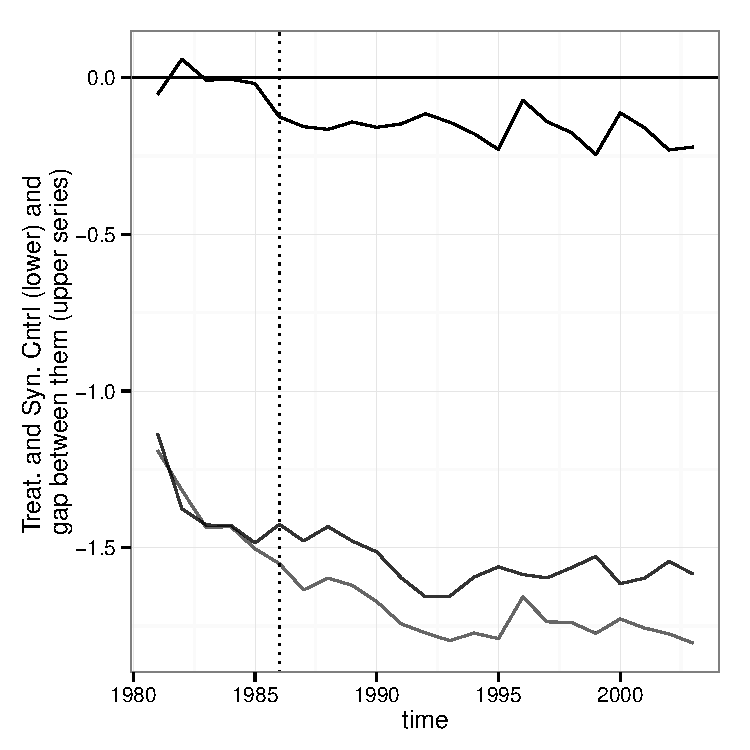
\includegraphics{img-gap-full.pdf}
      \caption{All covariates, all times}
      \label{fig:c11a}
    \end{subfigure}
    
    \begin{subfigure}[b]{\textwidth}
      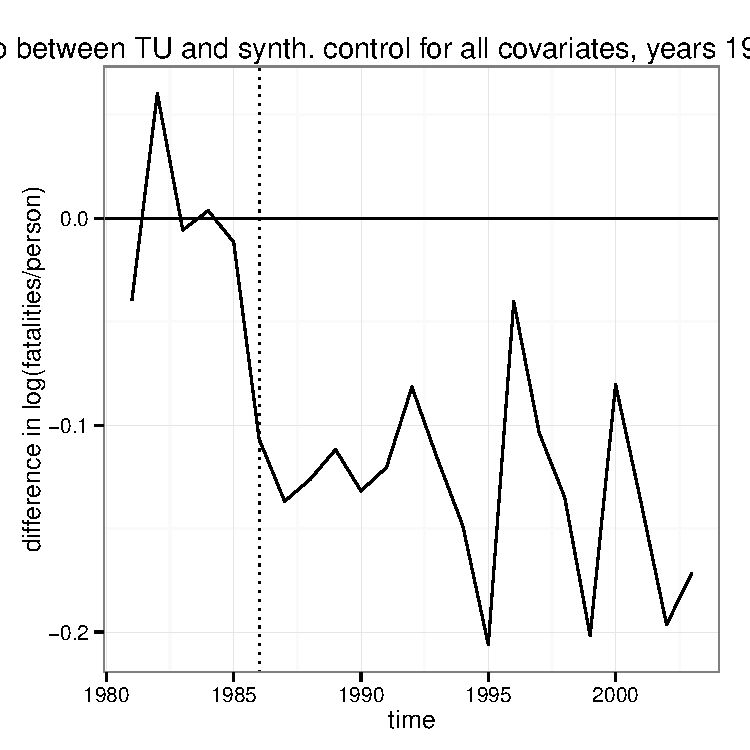
\includegraphics{img-gap-full1984.pdf}
      \caption{All covariates, 1981-1984}
      \label{fig:c11b}
    \end{subfigure}

    \begin{subfigure}[b]
      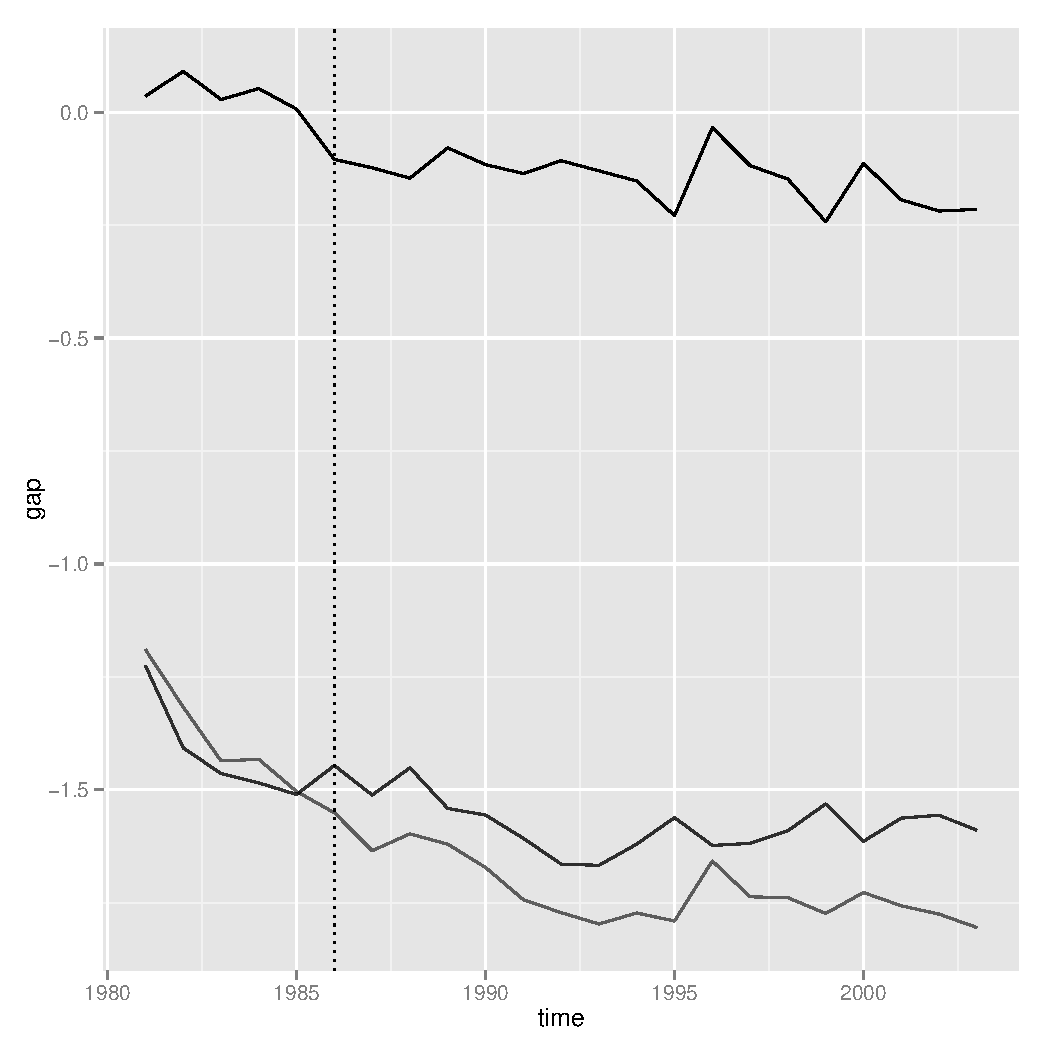
\includegraphics{img-gap-vmt.pdf}
      \caption{VMT per capita as covariate}
      \label{fig:c11c}
    \end{subfigure}
    \caption{Plots of gaps between Log(fatalities per capita) for synthetic control unit and treatment unit}\label{fig:c11}
\end{figure}


\begin{figure}
  \begin{centering}
    \begin{subfigure}[b]{\textwidth}
      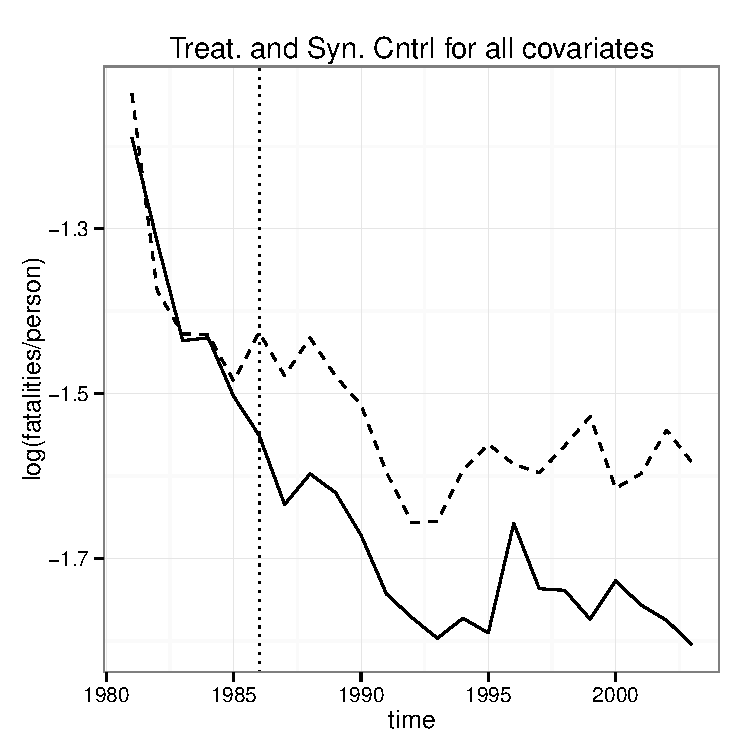
\includegraphics{img-split-full.pdf}
      \caption{All covariates, all times}
      \label{fig:c12a}
    \end{subfigure}

    \begin{subfigure}[b]{\textwidth}
      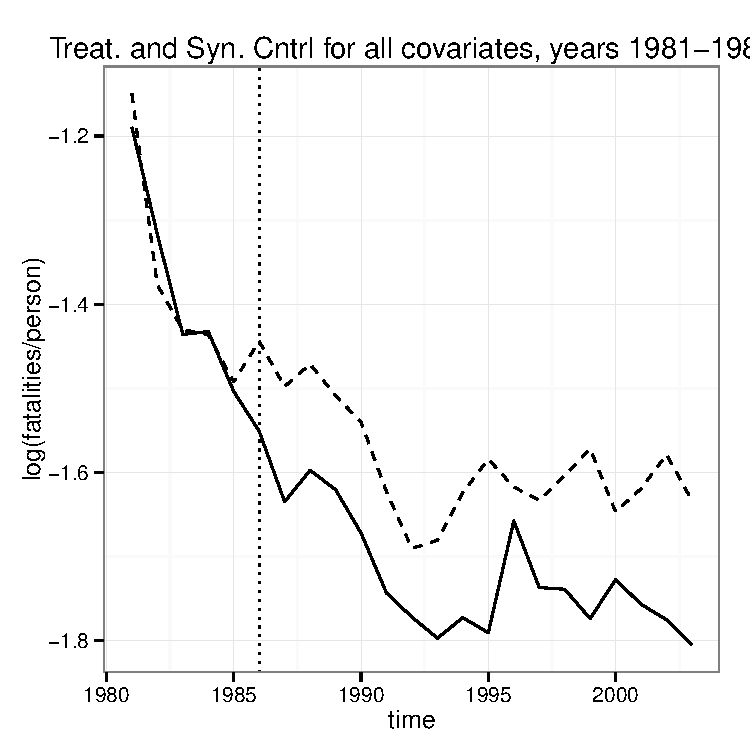
\includegraphics{img-split-full1984.pdf}
      \caption{All covariates, 1981-1984}
      \label{fig:c12b}
    \end{subfigure}

    \begin{subfigure}[b]
      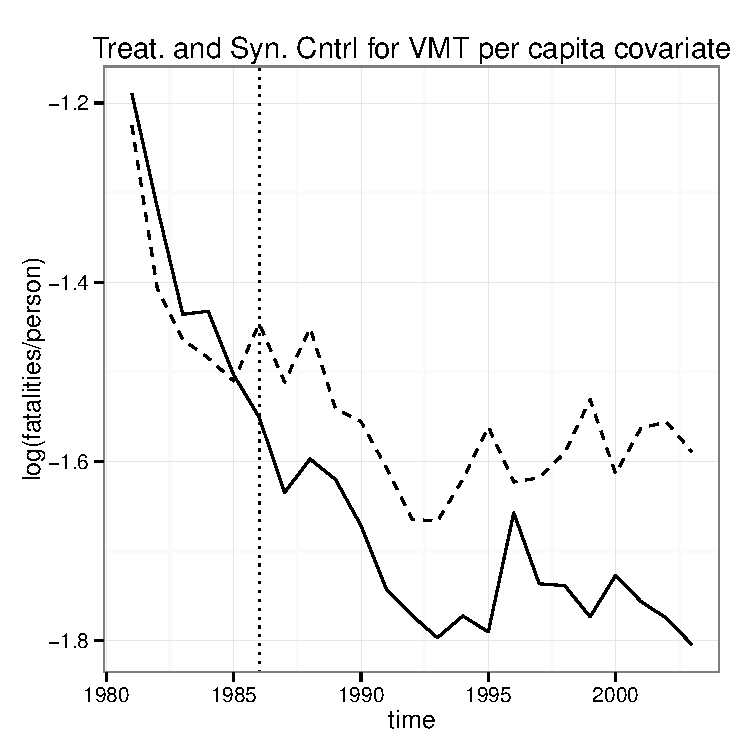
\includegraphics{img-split-vmt.pdf}
      \caption{VMT per capita as covariate}
      \label{fig:c12c}
    \end{subfigure}
    \caption{Plots of log(fatalities per capita) in synthetic control unit and treatment unit}\label{fig:c12}
\end{figure}


\subsection{Gap between TU \& preferred synth spec. and gap between each control state and its ``placebo'' treatment}

\paragraph{Graphical significance?}


\subsection{MSPE Ratios}

\paragraph{... Was it significant??}  We find that the MSPE ratio for the TU is about 20, which is the second highest among the combined set of the TU and the control states.  Florida (as a placebo) had a higher MSPE ratio, about 120.  This sows seeds of doubt but we still find that the TU has a higher apparent effect then 93\% of units.  


\section{Compare with FE Model}

Our central estimate for the impact of seatbelt laws using synthetic control methods is a 15\% reduction in fatality rate.  This is roughly double the estimates we found using a fixed effects model (8\% with significance at a 0.05 level) in the previous assignment.  It is notable that many of the alternative estimates for the coefficient on primary seatbelt laws had higher (but not significant) results closer to those we find with the synthetic controls method.  

The differences may stem from a reduced sample of treatment states in the synthetic control method.  Since only four states with primary seatbelt laws were included (out of nearly 20 that eventually have the laws) it could be the case that the analysis is biased.

Another source of difference is in the structural way the estimates are made.  Where the fixed effects model compares pre and post treatment, the synthetic controls method compares only in the post-treatment period.  The fixed effects model includes first and second order corrections for year which should address some of these issues, but to the extent that the trend in national-level drivers for traffic fatalities does not obey the quadratic functional form there are potential errors that are not present in the synthetic control method, since synthetic controls does not impose a linear function in the same way on the covariates.  

\section{Appendix: Code Listings}

\lstinputlisting{./ps2b.r}
\lstinputlisting{../util/are213-func.R}


\end{document}
